%%%%%%%%%%%%%%%%%%%%%%%%%%%%%%%%%%%%%%%%%
% Beamer Presentation
% LaTeX Template
% Version 1.0 (10/11/12)
%
% This template has been downloaded from:
% http://www.LaTeXTemplates.com
%
% License:
% CC BY-NC-SA 3.0 (http://creativecommons.org/licenses/by-nc-sa/3.0/)
%
%%%%%%%%%%%%%%%%%%%%%%%%%%%%%%%%%%%%%%%%%

%----------------------------------------------------------------------------------------
%	PACKAGES AND THEMES
%----------------------------------------------------------------------------------------

\documentclass{beamer}

\mode<presentation> {

% The Beamer class comes with a number of default slide themes
% which change the colors and layouts of slides. Below this is a list
% of all the themes, uncomment each in turn to see what they look like.

%\usetheme{default}
%\usetheme{AnnArbor}
%\usetheme{Antibes}
%\usetheme{Bergen}
%\usetheme{Berkeley}
%\usetheme{Berlin}
%\usetheme{Boadilla}
%\usetheme{CambridgeUS}
%\usetheme{Copenhagen}
%\usetheme{Darmstadt}
%\usetheme{Dresden}
%\usetheme{Frankfurt}
%\usetheme{Goettingen}
%\usetheme{Hannover}
%\usetheme{Ilmenau}
%\usetheme{JuanLesPins}
%\usetheme{Luebeck}
\usetheme{Madrid}
%\usetheme{Malmoe}
%\usetheme{Marburg}
%\usetheme{Montpellier}
%\usetheme{PaloAlto}
%\usetheme{Pittsburgh}
%\usetheme{Rochester}
%\usetheme{Singapore}
%\usetheme{Szeged}
%\usetheme{Warsaw}

% As well as themes, the Beamer class has a number of color themes
% for any slide theme. Uncomment each of these in turn to see how it
% changes the colors of your current slide theme.

%\usecolortheme{albatross}
%\usecolortheme{beaver}
%\usecolortheme{beetle}
%\usecolortheme{crane}
%\usecolortheme{dolphin}
%\usecolortheme{dove}
%\usecolortheme{fly}
%\usecolortheme{lily}
%\usecolortheme{orchid}
%\usecolortheme{rose}
%\usecolortheme{seagull}
%\usecolortheme{seahorse}
%\usecolortheme{whale}
%\usecolortheme{wolverine}

%\setbeamertemplate{footline} % To remove the footer line in all slides uncomment this line
\setbeamertemplate{footline}[page number] % To replace the footer line in all slides with a simple slide count uncomment this line

\setbeamertemplate{navigation symbols}{} % To remove the navigation symbols from the bottom of all slides uncomment this line
}

\usepackage{graphicx} % Allows including images
\usepackage{booktabs} % Allows the use of \toprule, \midrule and \bottomrule in tables
%\usepackage {tikz}
\usepackage{tkz-graph}
\GraphInit[vstyle = Shade]
\tikzset{
  LabelStyle/.style = { rectangle, rounded corners, draw,
                        minimum width = 2em, fill = yellow!50,
                        text = red, font = \bfseries },
  VertexStyle/.append style = { inner sep=5pt,
                                font = \normalsize\bfseries},
  EdgeStyle/.append style = {->, bend left} }
\usetikzlibrary {positioning}
%\usepackage {xcolor}
\definecolor {processblue}{cmyk}{0.96,0,0,0}
%----------------------------------------------------------------------------------------
%	TITLE PAGE
%----------------------------------------------------------------------------------------

\title[Short title]{Computational Astrophysics N-Body Project} % The short title appears at the bottom of every slide, the full title is only on the title page

\author{Benjamin Froelich} % Your name
\institute[UZH] % Your institution as it will appear on the bottom of every slide, may be shorthand to save space
{
University of Zuerich \\ % Your institution for the title page
\medskip
}
\date{\today} % Date, can be changed to a custom date

\begin{document}

\begin{frame}
\titlepage % Print the title page as the first slide
\end{frame}

\begin{frame}
\frametitle{Overview} % Table of contents slide, comment this block out to remove it
\tableofcontents % Throughout your presentation, if you choose to use \section{} and \subsection{} commands, these will automatically be printed on this slide as an overview of your presentation
\end{frame}

%----------------------------------------------------------------------------------------
%	PRESENTATION SLIDES
%----------------------------------------------------------------------------------------

%------------------------------------------------

\section{First Task}
\begin{frame}{Verification of Density function rho(r)}

\begin{figure}
	\centering
	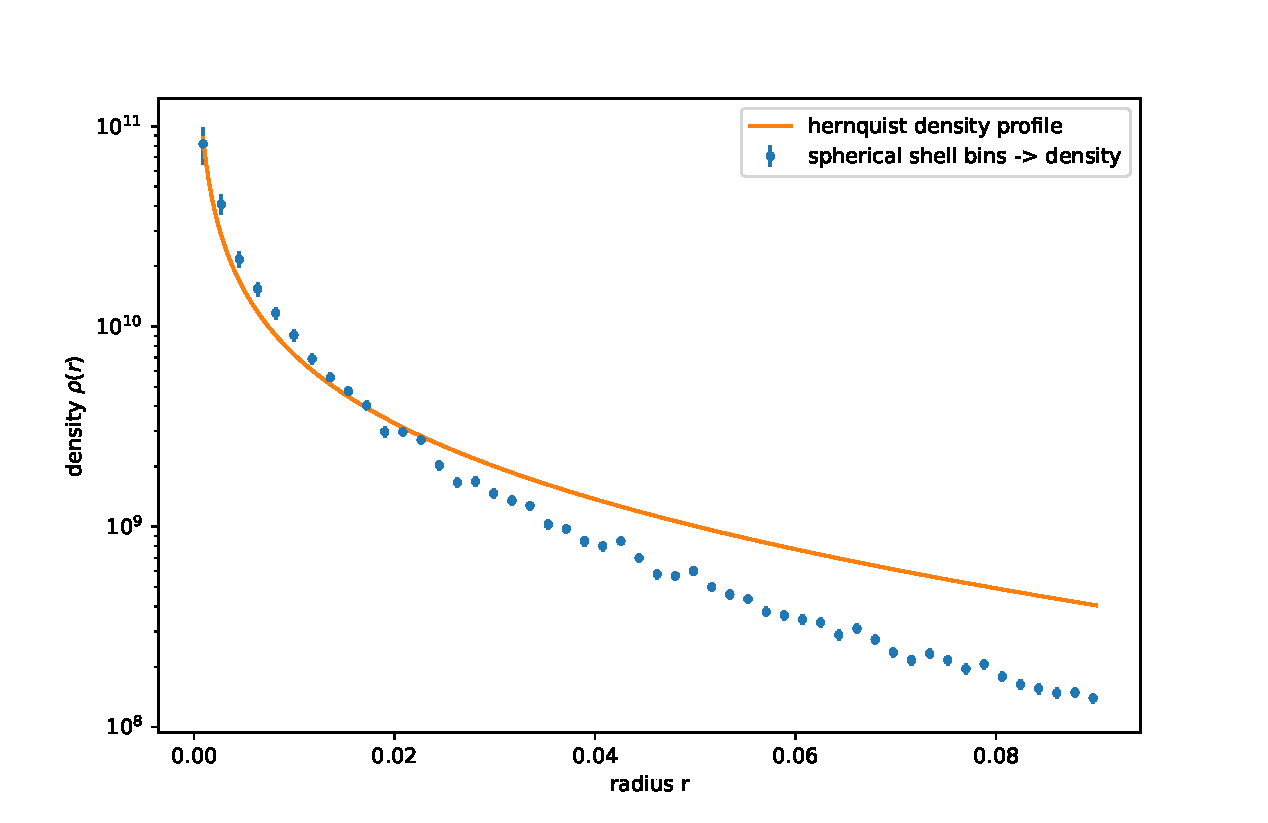
\includegraphics[width=0.8\linewidth]{hernquist1}
	\caption{hernquist density, scale parameter a $\approx$ 0.3017}
	\label{fig:hernquist1}
\end{figure}

\end{frame}

\begin{frame}{Unit Discussion}
	\begin{table}[H]
		\begin{tabular}{|c|c|c|c|}
			\hline 
			assuming & G=1 & l = 1 parsec & m = 1 jupiter mass \\ 
			\hline 
			SI & 6.6741e-11 $m^3 kg^{-1} s^{-2}$ &  3.086e16 $m$& 1.898e27 $kg$ \\ 
			\hline 
			factors& $\alpha = $6.6741e-11 & $\beta=$3.24e-17 & $\gamma=$5.27e-28 \\
			\hline
		\end{tabular} 
	\end{table}

	From
	\begin{equation}
		\alpha \frac{m^3}{s^2 kg} = G = 1
	\end{equation}

	unit of time follows
	$1s \hat{=} \sqrt{\alpha m^3 kg^{-1}} = \sqrt{\alpha \beta ^3 \gamma ^{-1}} $ $parsec ^{3/2} M_j ^{-1/2} $.
	Calculating back to SI units, velocity and time are:
	\begin{eqnarray}
		[t] = \sqrt{\alpha ^{-1} \beta ^{-3} \gamma} sec &
		[v] = \sqrt{\alpha \beta \gamma ^{-1}} \frac{m}{sec}
	\end{eqnarray}	
	
\end{frame}

\begin{frame}{Direct Force Calculation}
To find the analytical solution the following equation was used:
\begin{equation}
	a_{analytical}(r) = \frac{G}{r^2} \int_{0}^{r} 4 \pi \rho (r) r^2  dr  
\end{equation}

To solve the integral numerically with N particles:
\begin{equation}
	M(r) = \sum_{i, r_i < r}^N m_i   
\end{equation}

\end{frame}

\begin{frame}{Direct Force Calculation}
\begin{figure}
	\centering
	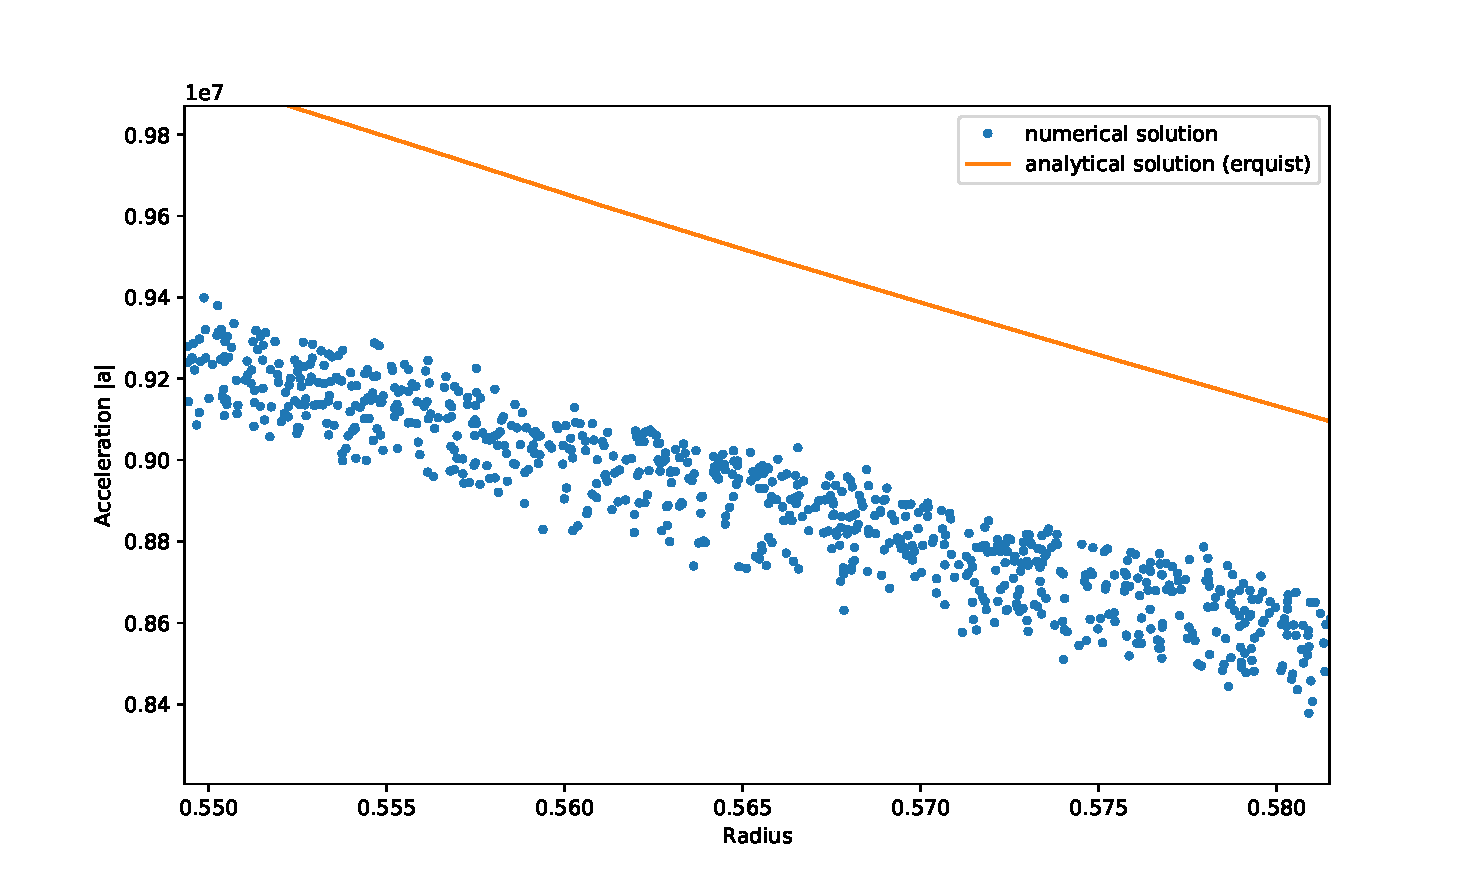
\includegraphics[width=1.0\linewidth]{hernquist3}
	\caption{Softening $\epsilon$ = 0.1}
	\label{fig:hernquist3}
\end{figure}
\end{frame}

\begin{frame}{Direct Force Calculation}
\begin{figure}
	\centering
	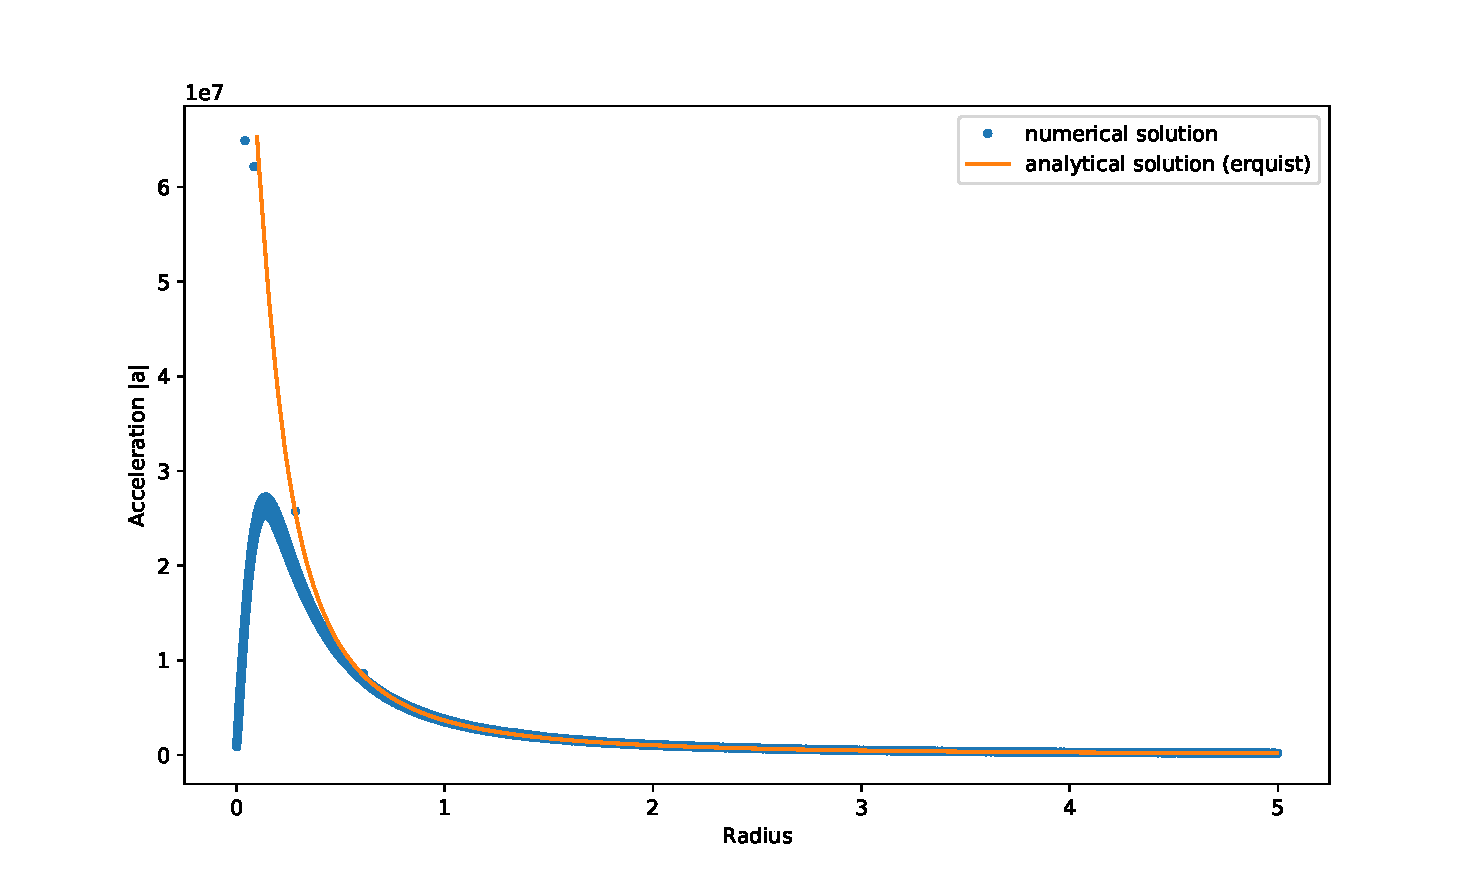
\includegraphics[width=1.0\linewidth]{hernquist2}
	\caption{Softening $\epsilon$ = 0.1}
	\label{fig:hernquist2}
\end{figure}
\end{frame}

\begin{frame}{Direct Force Calculation}
\begin{figure}
	\centering
	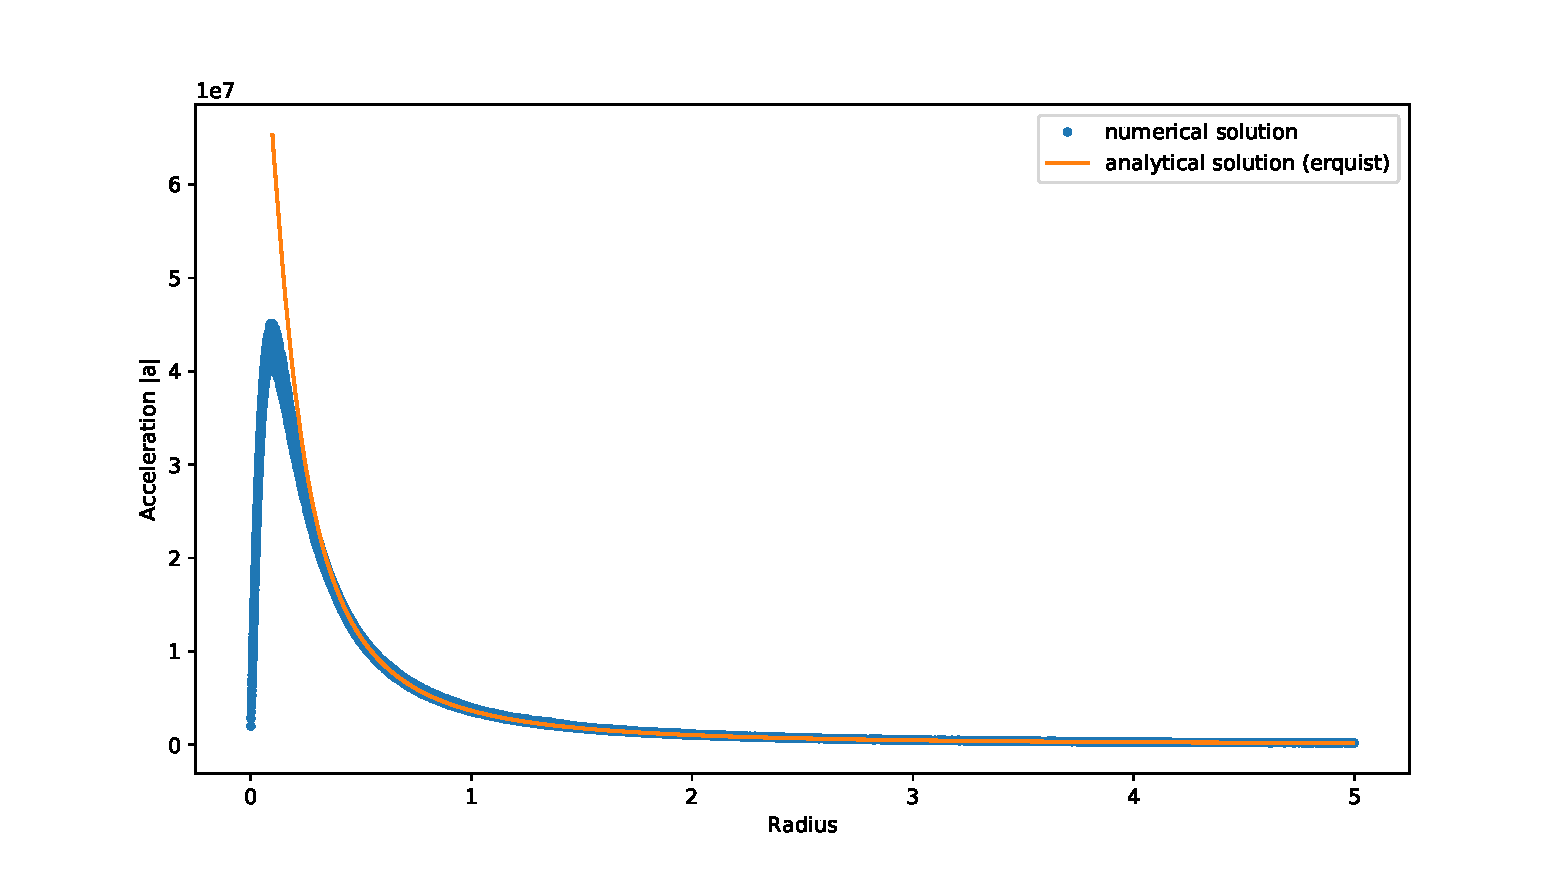
\includegraphics[width=1.0\linewidth]{hern_soft_05}
	\caption{Softening $\epsilon$ = 0.05}
	\label{fig:he3}
\end{figure}
\end{frame}

\begin{frame}{Time to relax}
	From lecture 4 and task description:
	\begin{eqnarray}
		t_{relax} = \frac{N}{8 \log{N}} t_{cross} \\
		v_c = \sqrt{\frac{G \cdot M(r < R_{hm})}{R_{hm}}}
	\end{eqnarray}

	
	To estimate $t_{cross}$:
	\begin{equation}
		v_c \approx \frac{R_{hm}}{t_{cross}} \rightarrow t_{cross} = \frac{R_{hm}}{v_{c}}
	\end{equation}
	
	
	
	\begin{equation}
		t_{relax}  = \frac{N}{8 \log N} \sqrt{\frac{R_{hm}^3}{G \cdot M(r < R_{hm})}}
	\end{equation}
	
	With N = 50010 from data we get $t_{relax} \approx 0.6905$.
	 Which is about 1.05e16 sec, 3.33e8 yrs! A higher softening leads to lower velocities, which leads to higher relaxation time.
	
	\end{frame}



\section{Second Task}
\begin{frame}{Direct force with softening}
	\begin{itemize}
		\item ok
		\item this
		\item is a test
	\end{itemize}
\end{frame}

\end{document}